\documentclass[a4paper,12pt]{article}

\usepackage[T1]{fontenc}
\usepackage{amsmath}
\usepackage{multicol}
\usepackage{enumitem}
\usepackage[margin=1cm,includefoot]{geometry}
\usepackage{tikzanim}
\usetikzlibrary{calc,intersections,tikzmark,decorations.pathreplacing}

\usepackage{hyperref}

\usepackage{listings}
\lstset{
	basicstyle=\ttfamily\footnotesize,
	columns=fullflexible,
	language={[LaTeX]TeX},
	tabsize=2,
	breaklines,
	xleftmargin=2em,
	backgroundcolor=\color{black!10},
	numbers=left,
	numberstyle=\color{black!50},
	commentstyle=\color{gray},
	keywordstyle=\color{teal!75!black},
	morekeywords={draw,coordinate,useasboundingbox},
	identifierstyle=\color{blue!75!black},
	emph={tikzanim,step,allframes,framepos},
	emphstyle=\color{purple},
	commentstyle=\color{green!75!black},
}

\tikzset{construct line/.style={densely dashed,black!25}}

\def\keywords{make easily animation with animate package and tikz}
\hypersetup{
  pdftitle={tikzanim's package},
  pdfsubject={Documentation},
  pdfauthor={Frédéric Bonnaud},
  pdfkeywords={\keywords},
    pdfborder = {0 0 0},
    colorlinks,
    citecolor=red,
    filecolor=Darkgreen,
    linkcolor=blue,
    urlcolor=cyan!50!black!90
}
\author{Frédéric Bonnaud}%
\title{\TikzAnimate\\ Create an animation with \Tikz}
\date{15th of july, 2020}

\newcommand\Tikz{{\ttfamily tikz}}
\newcommand\TikzAnimate{{\ttfamily tikzanim}}
\newcommand\Animate{{\ttfamily animate}}

\setlength{\parindent}{0mm}
\begin{document}

\maketitle

\tableofcontents

\bigskip

I apologie for my poor english.

\section{Introduction}

\TikzAnimate\ create animations in \LaTeX\ with  \Tikz\ and \Animate. Steps are drawn with standard \Tikz\ code. 

A \TikzAnimate's animation is made of steps. Each step draws transparencies which are uses with others to create frames of the part's step.

\section{\TikzAnimate's macros}

\subsection{\ttfamily\textbackslash tikzanim}

	This macro uses a {\ttfamily animateinline}'s environment, {\ttfamily\textbackslash multiframe} and a {\ttfamily tikzpicture}'s environment to prepare animationntes images).
	
	\textbf{Syntax~:} 
	
	\quad {\ttfamily \textbackslash tikzanim <overlay> [animateinline's options] \{frame rate\} [tikz's options] \{initialisation\} \\ \{steps\}}
	
	\begin{itemize}
		\item {\ttfamily <overlay>} : overlay number on which animation will be shown. Before this number, first frame of animation will be dran. After this number, last frame of animation will be drawn.
		
		\emph{Prefer a single number for the overlay, or animation will be render multiple times.}
		\item {\ttfamily [animateinline's options]} : options which are pass to {\ttfamily animateinline}'s environment.
		
		Défault value : {\ttfamily poster=last,controls}
		\item {\ttfamily \{frame rate\}} : the starting frame rate. Each step can change it.
		\item {\ttfamily [options tikz]} : options which are pass to {\ttfamily tikzpicture}'s environment.
		
		Défault value : no option
		\item {\ttfamily \{initialisation\}} : \Tikz's code. This code will initialize all frames. Minimaly, it should call {\ttfamily\textbackslash useasboundingbox} to
		set same size to all transparencies.
		\item {\ttfamily \{étapes\}} : list of steps. 
	\end{itemize}
	
\subsection{\ttfamily\textbackslash step}

	This macro define a new animation's step. \Animate\ uses a transparencies' stack. Each animation's frame is draw by showing all the stack.
	{\ttfamily\textbackslash step} manage the stack and frame frame creation.
	
	At start, the stack is empty. A {\ttfamily\textbackslash step} call will :
	
	\begin{enumerate}[label=(\arabic*)]
		\item create first image of the step, put it on the stack for a frame.
		\item \tikzmark{boucle}remove last image of the stack.
		\item create next image, put it on the stack for a frame.
		\item \tikzmark{test}If it's not step's end, go to (2).
		\item If it's step's end, last image will stay on stack for some define time.
		
	\end{enumerate}
	\begin{tikzpicture}[remember picture,overlay]
		\coordinate(T)at(-10mm,1mm);
		\draw[-latex,thick] ($(pic cs:test)+(T)$) to[bend left] ($(pic cs:boucle)+(T)$) ; 
	\end{tikzpicture}
	
	\textbf{Syntaxe :}
	
	\quad {\ttfamily\textbackslash step[*] [frame rate] \{images\} [duration] \{tikz' code\} }
	
	\begin{itemize}
		\item {\ttfamily *} : star version will clear transparencies stack at animation's start.
		\item {\ttfamily[frame rate]} : define the new frame rate.
		
		Défault value : last frame rate defined either by {\ttfamily\textbackslash tikzanim} or {\ttfamily\textbackslash step}.
		\item {\ttfamily\{images\}} : define how many frames {\ttfamily\textbackslash step} will define. If 0, a transparencies is created but no frame. The transparencies will last for {\ttfamily[duration]} on the stack.
		
		\item {\ttfamily[duration]} : set duration of last step's transparency (in frames).
		
		Défault value : 0, to animation's end.
		
		\item {\ttfamily\{tikz's code\}} : here goes \Tikz's code which will draw each transparency. This code should use all previous initialised code,
		and, to make things depends on which frame is to be drawn, the macros {\ttfamily\textbackslash framepos} and {\ttfamily\textbackslash iframe}.
		
		\begin{itemize}
			\item The macro {\ttfamily\textbackslash framepos} is set to 0 at step's start, and will go to 1 at step's end. {\ttfamily\textbackslash step} will set this macro.
			\item The macro {\ttfamily\textbackslash iframe} is set to transparency number. {\ttfamily\textbackslash multiframe} from \Animate's package will set this macro.
		\end{itemize}
		
	\end{itemize}
	
	\begin{multicols}{2}
	{Le code suivant~:}
	\begin{lstlisting}
% \usepackage{tikzanim}
\tikzanim{10}{
	\useasboundingbox(0,0)rectangle(5,2.5) ;
}{	
	% this step will last 15 frames
	% this is half next step's duration
	\step{30}[15]{
		% we need to initialize boundingbox
		\coordinate(A)at(0,0) ;
		\coordinate(B)at(5,2.5) ;
	}{
		\draw(A)--($(A)!\framepos!(B)$) ;
	}
	% next step will be 2 times speeder
	\step[20]{30}{
		% no initialisation, C and D
		% won't be use next
	}{
		\coordinate(C)at(0,2.5) ;
		\coordinate(D)at(5,0) ;
		\draw(C)--($(C)!\framepos!(D)$) ;
	}
}
	\end{lstlisting}
	
	{Make this animation~:}
	
	\bigskip
	
	\centering
	% \usepackage{tikzanim}
	\tikzanim{10}{
		\useasboundingbox(-0.1,0.1)rectangle(5.1,2.6) ;
	}{
		\step{30}[15]{
			\coordinate(A)at(0,0) ;
			\coordinate(B)at(5,2.5) ;
			\draw(A)--($(A)!\framepos!(B)$) ;
		}
		\step[20]{30}{
			% pas d'initialisation, C et D ne
			% sont pas utilisés par la suite
			\coordinate(C)at(0,2.5) ;
			\coordinate(D)at(5,0) ;
			\draw(C)--($(C)!\framepos!(D)$) ;
		}
	}
	
	\end{multicols}
	
	\textbf{How does the stack work~:}
	
	\medskip
	
\newcounter{dy} 
\newcommand{\transparentlist}[2]{
	\stepcounter{dy}	
	\foreach\f in {#1}{
		\pgfmathsetmacro{\c}{\f*5}
		\path[draw=black,fill=teal!\c!purple!75!white,fill opacity=0.75] (\f*0.1,-\thedy*0.8)node(a){} -- ++(0,0.6) -- ++(0.3,0.3)node(b){} -- ++(0,-0.6) -- cycle ;
		\path(a)--node[midway,font=\tiny,shape=rectangle]{\f} (b) ;
	}
	\node[anchor=west,shape=rectangle] at(2.5,0.4-\thedy*0.8) {#2#1} ;
}

\newcommand{\acc}[4][0pt]{
		\draw[decorate,decoration={brace,amplitude=10pt},thick,xshift=#1] (12,-0.8*#2-0.05) --node[right,xshift=10pt,text width=7cm,font=\ttfamily,shape=rectangle]{#4} (12,-0.8*#3+0.05);
}

\newcommand{\entoure}[4][red,thick,densely dashed]{
	\filldraw[red,thick,densely dashed,fill opacity=0.333,#1] (#2*0.1-0.05,-#4*0.8-0.125) -- ++(0,{(#4-#3+1)*0.8-0.05}) -- ++(0.4,0.4) -- ++ (0,{-(#4-#3+1)*0.8+0.05}) -- cycle	;
}

\newcommand{\limite}[2][teal!50,thick,densely dotted]{
	\draw[#1](-0.2,-0.8*#2) -- (11.9,-0.8*#2) ;
}


\begin{tikzpicture}[shape=coordinate]

	\entoure{0}{1}{18}

	%\def\label{Liste de transparents : }
	%\transparentlist{0,...,20}{\label}
	\def\label{Frame \thedy, make of transparencies~: }
	
	\transparentlist{0,1}{\label}
	\transparentlist{0,2}{\label}
	\transparentlist{0,3}{\label}
	\transparentlist{0,4}{\label}
	\transparentlist{0,5}{\label}
	
	\entoure{6}{6}{9}
	
	\transparentlist{0,6}{\label}
	
	\acc{0}{6}{ 
		\textbackslash step\{0\}{\color{red}[18]}\{...\}\\ 
		{\rmfamily add 1 transparency lasting 18 images, no image is added}\\
		\textbackslash step\{6\}{\color{red}[4]}\{...\}\\
		{\rmfamily add 6 transparencies and 6 images, last will last 4 images}
	}
	
	\limite{6}
	
	\transparentlist{0,6,7}{\label}
	\transparentlist{0,6,8}{\label}
	\transparentlist{0,6,9}{\label}
	\transparentlist{0,10}{\label}
	\transparentlist{0,11}{\label}

	\acc{6}{11}{ 
		\textbackslash step\{5\}\{...\} \\
		{\rmfamily add 5 transparencies and 5 images}
	}
	
	\limite{11}
	
	\transparentlist{0,11,12}{\label}
	\transparentlist{0,11,13}{\label}
	\transparentlist{0,11,14}{\label}
	\transparentlist{0,11,15}{\label}
	\entoure{16}{16}{18}
	\transparentlist{0,11,16}{\label}
	
	\acc{11}{16}{
		\textbackslash step\{5\}{\color{red}[3]}\{...\} \\
		{\rmfamily add 5 transparencies and 5 images, last will last 3 images}
	}
	
	\limite{16}
	
	\transparentlist{0,11,16,17}{\label}
	\transparentlist{0,11,16,18}{\label}
	\transparentlist{11,19}{\label}
	\transparentlist{11,20}{\label}
	
	\acc{16}{20}{
		\textbackslash step\{4\}\{...\} \\
		{\rmfamily add 4 transparencies and 4 images}
	}

\end{tikzpicture}
	

\subsection{\ttfamily\textbackslash allframes}

This macro draw on all transparencies.

\textbf{Syntax~:}

\quad {\ttfamily\textbackslash allframes \{tikz's code\}}

	\begin{itemize}
		\item {\ttfamily\{tikz's code\}} : set \Tikz's code to be drawn on each transparency chargé de dessiner sur tous les transparents. This code should use all previous initialised code,
		{\ttfamily\textbackslash framepos} and {\ttfamily\textbackslash iframe}.
	\end{itemize}
	
\section{\ttfamily timeline}

\Animate\ ues a {\ttfamily timeline} file to manage transparencies' stack. \TikzAnimate\ will create a {\ttfamily timeline} file by animation. They are named~: {\ttfamily \textbackslash jobname.tzc\#.tln}. You can use them for debug purpose.
	
\section{A complet sample}

\begin{lstlisting}[name=exemplecomplet]
\gdef\aLen{5}
\gdef\bLen{2}
\pgfmathsetmacro{\cLen}{sqrt(\aLen^2+\bLen^2)}
\tikzset{bleu/.style={fill=blue!30,fill opacity=0.5},rouge/.style={fill=red!30,fill opacity=0.5}} 
\end{lstlisting}

Some initialisations.


\begin{lstlisting}[name=exemplecomplet]

\tikzanim[poster=0,controls]{1}{
	% initialisation 
	\useasboundingbox(-0.1,-\bLen-0.1)rectangle(\aLen+\bLen+0.1,\aLen+0.1) ;
}	
\end{lstlisting}

Animation will start at 1 frame by seconde.

Then we create helping construction points and a transparency which will not create a frame. It only show on first frame.

\begin{lstlisting}[name=exemplecomplet]
{
	\step{0}[1]{		
		\coordinate(A)at(0,0) ;
		\coordinate(B)at(\aLen,0) ;
		\coordinate(C)at(\aLen,\aLen) ;
		\coordinate(D)at(0,\aLen) ;

		\coordinate(E)at(\aLen+\bLen,0) ;
		\coordinate(F)at(\aLen+\bLen,\bLen) ;
		\coordinate(G)at(\aLen,\bLen) ;

		\path[name path=EC](E)--(C) ;
		\path[name path=FG](F)--(G) ;
		\path[name intersections={of=EC and FG,by=H}] ;

		\coordinate(I)at(0,\aLen-\bLen) ;
		\coordinate(J)at($(A)+(H)-(G)$);
		% first triangle
		\fill[bleu] (C) -- (D) -- (I) -- cycle ;
	}
\end{lstlisting}

We create a new transparency will be shown on next frame to end of the 4th step after this one.

\begin{lstlisting}[name=exemplecomplet]
	\step{0}[4.0]{
		% second triangle
		\fill[bleu] (I) -- (A) -- (J) -- cycle ;
	}
\end{lstlisting}

We create a new transparency will be shown on next frame to the end of the 5th step after this one.

\begin{lstlisting}[name=exemplecomplet]
	\step{0}[5.0]{
		% third triangle
		\fill[rouge] (E) -- (F) -- (H) -- cycle ;
	}
\end{lstlisting}

Then we create one transparency which will be shown for all next ones containing fixed stuff and the 3 first transparencies.

\begin{lstlisting}[name=exemplecomplet]
	\step{1}{
		% starting figure
		\draw (A) -- (B) -- (C) -- (D) --cycle ;
		\draw (B) -- (E) -- (F) -- (G) --cycle ;
		
		\fill[bleu] (I) -- (J) -- (B) -- (C) -- cycle ;
		\draw (J) -- (B) -- (C) ; \draw[densely dotted] (C) -- (I) -- (J) ;
			
		\fill[rouge] (B) -- (E) -- (H) -- (G) -- cycle ;
		\draw (H) -- (G) -- (B) -- (E) ; \draw[densely dotted] (E) -- (H) ;
	}
\end{lstlisting}

First moving step at a frame rate of 5 images by second, for 10 transparencies, last will be lasting 1 image.

\begin{lstlisting}[name=exemplecomplet]
	% first triangle moves :
	\step[5]{10}[1]{
		\coordinate(M)at($(C)!\framepos!(E)$);% Point at \framepos on [CE]
		\coordinate(CM)at($(M)-(C)$) ;
		\coordinate(ICM)at($(I)+(CM)$);
		\coordinate(CCM)at($(C)+(CM)$);
		\coordinate(DCM)at($(D)+(CM)$);
		\coordinate(S)at(barycentric cs:I=1,C=1,D=1);
		\coordinate(S')at(barycentric cs:ICM=1,CCM=1,DCM=1);
		\fill[bleu] (ICM) -- (CCM) -- (DCM) -- cycle ;
		\draw[densely dotted] (ICM) -- (CCM) ;
		\draw (CCM) -- (DCM) -- (ICM) ;
		\draw[-latex](S)--(S') ;
	}
\end{lstlisting}

We draw only triangle on last position (not the arrow).

\begin{lstlisting}[name=exemplecomplet]
	% final postion
	\step{1}{
		\fill[bleu] (ICM) -- (CCM) -- (DCM) -- cycle ;
		\draw[densely dotted] (ICM) -- (CCM) ;
		\draw (CCM) -- (DCM) -- (ICM) ;
	}
\end{lstlisting}

We do the same for the second triangle.

\begin{lstlisting}[name=exemplecomplet]
	% second triangle moves
	\step{10}[1]{
		\coordinate(N)at($(I)!\framepos!(C)$);% Point at \framepos on [IC]
		\coordinate(IN)at($(N)-(I)$) ;
		\coordinate(IIN)at($(I)+(IN)$);
		\coordinate(JIN)at($(J)+(IN)$);
		\coordinate(AIN)at($(A)+(IN)$);
		\coordinate(T')at(barycentric cs:IIN=1,JIN=1,AIN=1);
		\fill[bleu] (IIN) -- (JIN) -- (AIN) -- cycle ;
		\draw[densely dotted] (IIN) -- (JIN) ;
		\draw (JIN) -- (AIN) -- (IIN) ;
		\draw[-latex](T)--(T') ;
	}
	% final position 
	\step{1}{
		\fill[bleu] (IIN) -- (JIN) -- (AIN) -- cycle ;
		\draw[densely dotted] (IIN) -- (JIN) ;
		\draw (JIN) -- (AIN) -- (IIN) ;
	}
 \end{lstlisting}
 
 We do the same for the third triangle.

 \begin{lstlisting}
	% third tiangle moves
	\step{10}[1]{
		\coordinate(P)at($(H)!\framepos!(J)$);% Point at \framepos on [HJ]
		\coordinate(HP)at($(P)-(H)$) ;
		\coordinate(EHP)at($(E)+(HP)$);
		\coordinate(FHP)at($(F)+(HP)$);
		\coordinate(HHP)at($(H)+(HP)$);
		\coordinate(U)at(barycentric cs:E=1,F=1,H=1);
		\coordinate(U')at(barycentric cs:EHP=1,FHP=1,HHP=1);
		\fill[rouge] (EHP) -- (FHP) -- (HHP) -- cycle ;
		\draw[densely dotted] (EHP) -- (HHP) ;
		\draw (EHP) -- (FHP) -- (HHP) ;
		\draw[-latex](U)--(U') ;
	}
	% final position
	\step{1}{
		\fill[rouge] (EHP) -- (FHP) -- (HHP) -- cycle ;
		\draw[densely dotted] (EHP) -- (HHP) ;
		\draw (EHP) -- (FHP) -- (HHP) ;
	}
}
\end{lstlisting}

\textbf{The animation :}

A visual proof of Pythagore's theorem.

\begin{center}
\gdef\aLen{5}
\gdef\bLen{2}
\pgfmathsetmacro{\cLen}{sqrt(\aLen^2+\bLen^2)}
\tikzset{bleu/.style={fill=blue!30,fill opacity=0.5},rouge/.style={fill=red!30,fill opacity=0.5}} 

\tikzanim[poster=0,controls]{5}[>=latex,inner sep=2pt]{
	\useasboundingbox(-0.75,-\bLen-0.75)rectangle(\aLen+\bLen+0.75,\aLen+0.75) ;
}{
	\step[1]{0}[1]{
		
		\coordinate(A)at(0,0) ;
		\coordinate(B)at(\aLen,0) ;
		\coordinate(C)at(\aLen,\aLen) ;
		\coordinate(D)at(0,\aLen) ;
		
		\coordinate(E)at(\aLen+\bLen,0) ;
		\coordinate(F)at(\aLen+\bLen,\bLen) ;
		\coordinate(G)at(\aLen,\bLen) ;

		\path[name path=EC](E)--(C) ;
		\path[name path=FG](F)--(G) ;
		\path[name intersections={of=EC and FG,by=H}] ;

		\coordinate(I)at(0,\aLen-\bLen) ;
		\coordinate(J)at($(A)+(H)-(G)$);
		\fill[bleu] (C) -- (D) -- (I) -- cycle ;
		
		\path(A) --node{$a^2$} (C) ;
		\path(E) --node{$b^2$} (G) ;
		
	}
	\step{0}[4.0]{
		\fill[bleu] (I) -- (A) -- (J) -- cycle ;
	}
	\step{0}[5.0]{
		\fill[rouge] (E) -- (F) -- (H) -- cycle ;
	}
	\step{1}{
		\draw[blue,line width=2pt] (A) -- (B) -- (C) -- (D) --cycle ;
		\draw[red,line width=2pt] (B) -- (E) -- (F) -- (G) --cycle ;
		
		\fill[bleu] (I) -- (J) -- (B) -- (C) -- cycle ;
		\draw (J) -- (B) -- (C) ; \draw[densely dotted] (C) -- (I) -- (J) ;
			
		\fill[rouge] (B) -- (E) -- (H) -- (G) -- cycle ;
		\draw (H) -- (G) -- (B) -- (E) ; \draw[densely dotted] (E) -- (H) ;
		
		\draw[<->]($(I)-(0.3,0)$)--node[fill=white]{$b$} ($(D)-(0.3,0)$) ;
		\draw[<->]($(D)+(0,0.3)$)--node[fill=white]{$a$} ($(C)+(0,0.3)$) ;
		\draw[<->]($(E)+(0.3,0)$)--node[fill=white]{$b$} ($(F)+(0.3,0)$) ;
		
	}

	\step[5]{10}[1]{
		\coordinate(M)at($(C)!\framepos!(E)$);% Point à \framepos sur [CE]
		\coordinate(CM)at($(M)-(C)$) ;
		\coordinate(ICM)at($(I)+(CM)$);
		\coordinate(CCM)at($(C)+(CM)$);
		\coordinate(DCM)at($(D)+(CM)$);
		\coordinate(S)at(barycentric cs:I=1,C=1,D=1);
		\coordinate(S')at(barycentric cs:ICM=1,CCM=1,DCM=1);
		\fill[bleu] (ICM) -- (CCM) -- (DCM) -- cycle ;
		\draw[densely dotted] (ICM) -- (CCM) ;
		\draw (CCM) -- (DCM) -- (ICM) ;
		\draw[->](S)--(S') ;
	}
	
	\step{1}{
		\fill[bleu] (ICM) -- (CCM) -- (DCM) -- cycle ;
		\draw[densely dotted] (ICM) -- (CCM) ;
		\draw (CCM) -- (DCM) -- (ICM) ;
	}
	
	\step{10}[1]{
		\coordinate(N)at($(I)!\framepos!(C)$);% Point à \framepos sur [IC]
		\coordinate(IN)at($(N)-(I)$) ;
		\coordinate(IIN)at($(I)+(IN)$);
		\coordinate(JIN)at($(J)+(IN)$);
		\coordinate(AIN)at($(A)+(IN)$);
		\coordinate(T)at(barycentric cs:I=1,J=1,A=1);
		\coordinate(T')at(barycentric cs:IIN=1,JIN=1,AIN=1);
		\fill[bleu] (IIN) -- (JIN) -- (AIN) -- cycle ;
		\draw[densely dotted] (IIN) -- (JIN) ;
		\draw (JIN) -- (AIN) -- (IIN) ;
		\draw[->](T)--(T') ;
	}
	
	\step{1}{
		\fill[bleu] (IIN) -- (JIN) -- (AIN) -- cycle ;
		\draw[densely dotted] (IIN) -- (JIN) ;
		\draw (JIN) -- (AIN) -- (IIN) ;
	}
	
	\step{10}[1]{
		\coordinate(P)at($(H)!\framepos!(J)$);% Point à \framepos sur [HJ]
		\coordinate(HP)at($(P)-(H)$) ;
		\coordinate(EHP)at($(E)+(HP)$);
		\coordinate(FHP)at($(F)+(HP)$);
		\coordinate(HHP)at($(H)+(HP)$);
		\coordinate(U)at(barycentric cs:E=1,F=1,H=1);
		\coordinate(U')at(barycentric cs:EHP=1,FHP=1,HHP=1);
		\fill[rouge] (EHP) -- (FHP) -- (HHP) -- cycle ;
		\draw[densely dotted] (EHP) -- (HHP) ;
		\draw (EHP) -- (FHP) -- (HHP) ;
		\draw[->](U)--(U') ;
	}
	
	\step{1}{
		\fill[rouge] (EHP) -- (FHP) -- (HHP) -- cycle ;
		\draw[densely dotted] (EHP) -- (HHP) ;
		\draw (EHP) -- (FHP) -- (HHP) ;
	}
	\step{1}{
		\draw[line width=2pt] (C) -- (I) -- (EHP) -- (E) -- cycle ;
		\draw[<->] ($(I)!0.3/\cLen!(EHP)$) --node[fill=blue!15]{$c$} ($(C)!0.3/\cLen!(E)$) ;
		\path (EHP) -- node{${\color{blue}a^2} + {\color{red}b^2} = c^2$} (C) ;
	}
}
\end{center}

\end{document}
